\chapter{Evaluation and Results}
\label{ch:evaluation-and-results}

\section{Over-, Under-Allocation of Data}
\label{sec:over-under-allocation-of-data}

  placeholder

\section{Trace Data}
\label{sec:data-analysis-evaluation}

  % \subsection{Structure of the Trace Data}
  This section contains the analysis of the Alibaba datasets that are used in section \ref{sec:evaluation-setup}. This data analysis builds on top of data analysis done in \cite{fengcunDeepJSJobScheduling2023}.
  Alibaba provides numerous monitoring traces clustered in different data clusters collected in a GitHub repository \cite{wengAlibabaClusterTrace2023}.
  For the evaluation of the prediction performance of the LSTM model configurations, the GPU cluster dataset \texttt{cluster-trace-gpu-v2020} was chosen. Analysis and characterisation of the GPU cluster data were done in \cite{wengMLaaSWildWorkload2022}.
  The data structure of the monitoring traces is shown in figure \ref{fig:gpu-trace-data-structure}, where a job consists of multiple tasks that get deployed on one or more instances depending on the defined number of instances.

  \begin{figure}
    \centering
    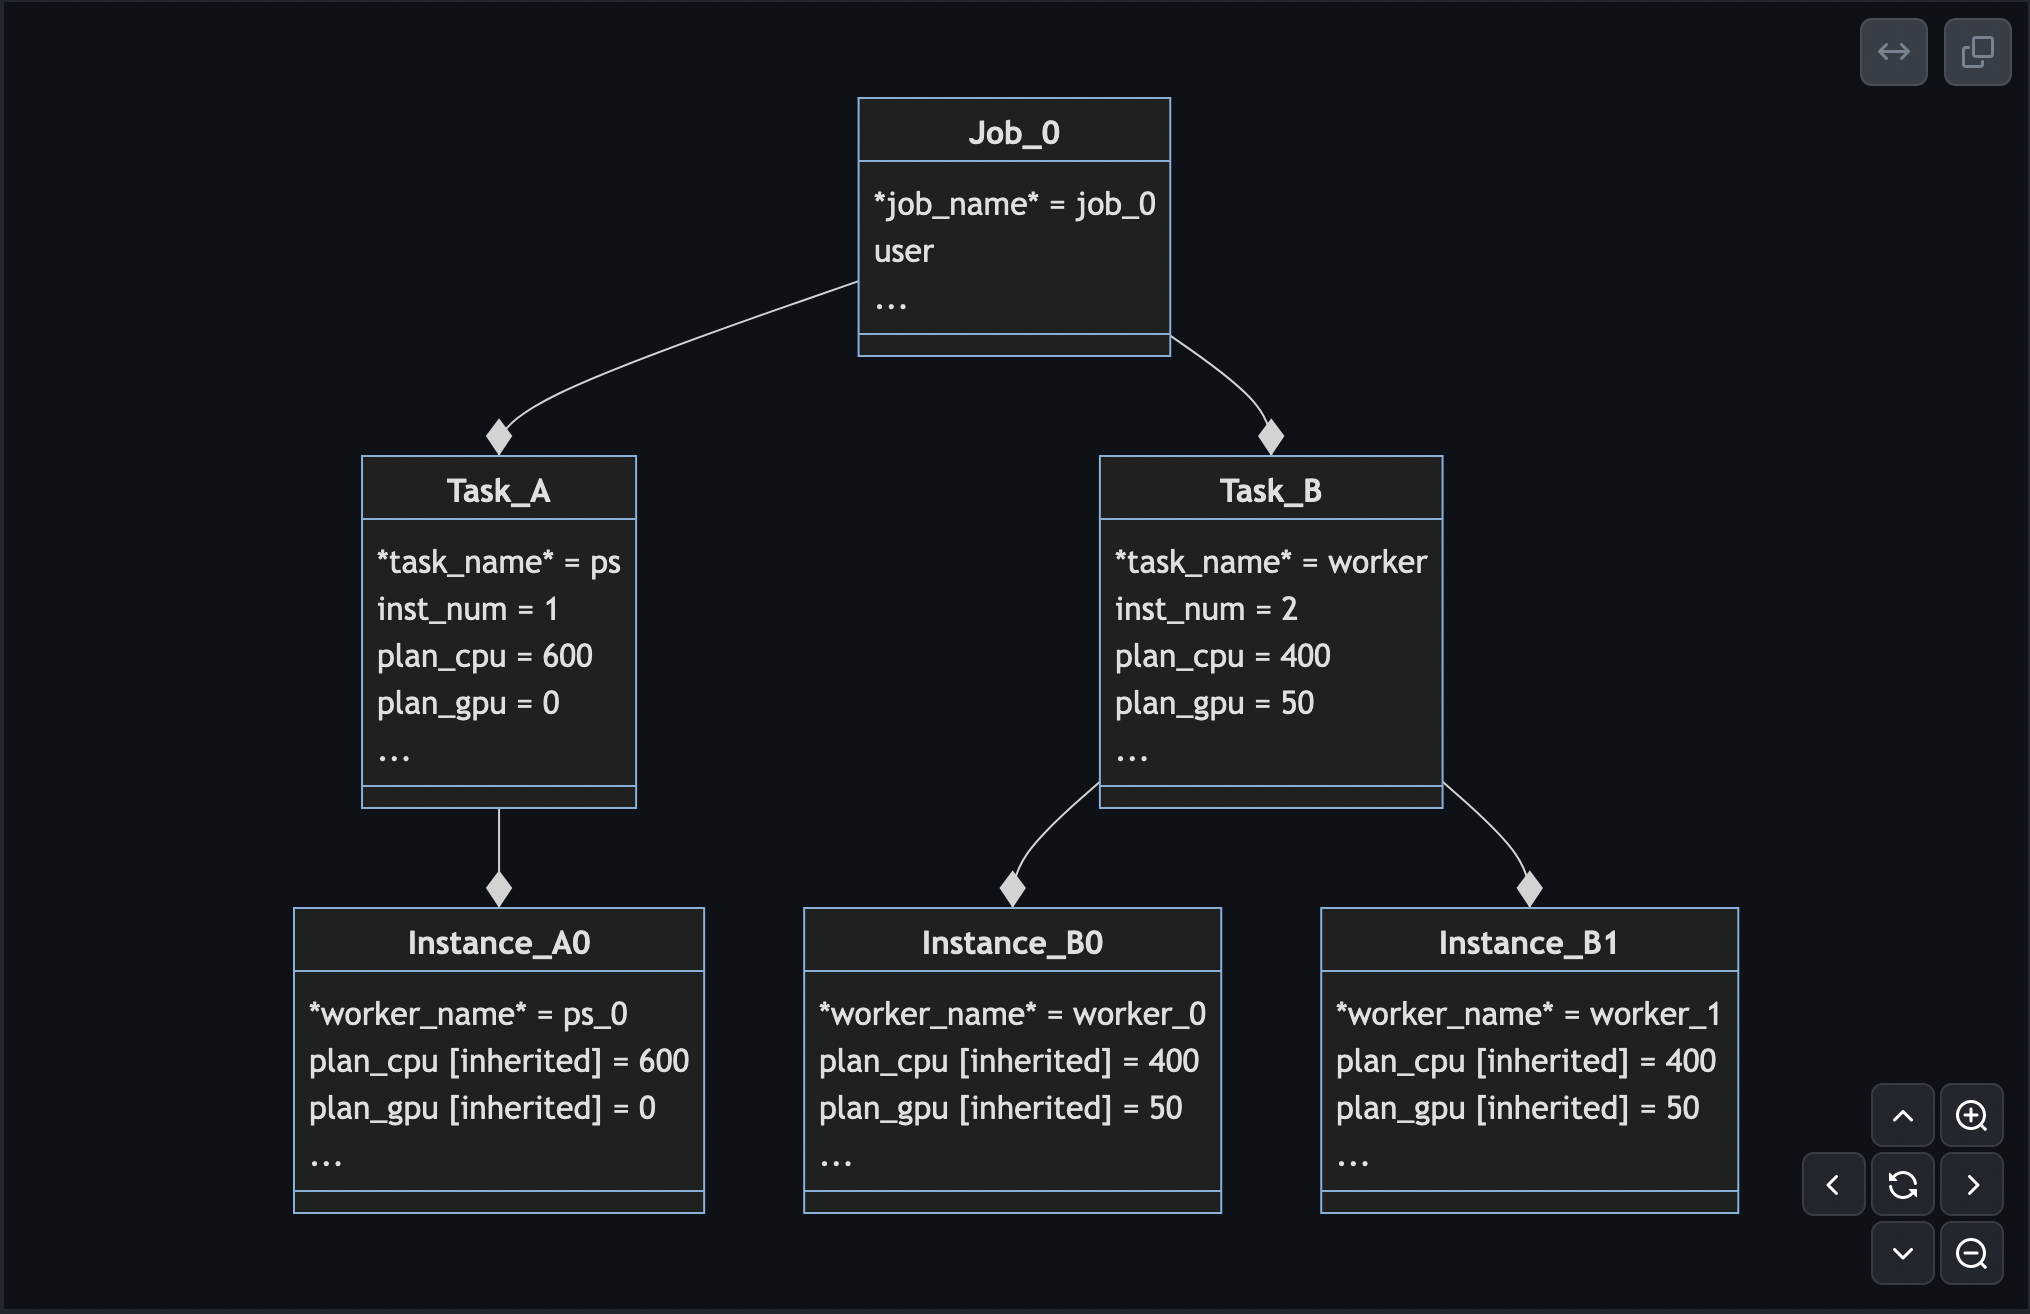
\includegraphics[width=0.95\textwidth]{figures/gpu_dataset_structure.png}
    \caption{GPU Trace Data Structure \cite{wengClusterdataClustertracegpuv2020Master}}
    \label{fig:gpu-trace-data-structure}
  \end{figure}
  

  \subsection{CPU Data Analysis}
  \label{sec:cpu-data-analysis}

    In table \ref{tab:actual-cpu-utilisation} the actual CPU utilisation of all tasks is shown.
    The dataset contains $5000$ elements and the CPU utilisation is represented in percentage, 
    thus a CPU utilisation of $200$ states that a task utilised two full CPU cores on average.
    \begin{table}
      \centering
      \caption{Actual CPU Utilisation}
      \label{tab:actual-cpu-utilisation}
      \begin{tabular}{|l|r|}
        \toprule
        {} &  CPU Utilisation (in \%) \\
        \midrule
        mean  &    516.073 \\
        std   &    881.832 \\
        min   &      1.023 \\
        25\%   &    103.632 \\
        50\%   &    208.749 \\
        75\%   &    528.076 \\
        max   &   7790.371 \\
        \bottomrule
      \end{tabular}
    \end{table}
    The mean of the CPU utilisation in this dataset is $516.073$, 
    so on average, a task required $516.073$ CPU utilisation, or $5.16$ CPU cores for its execution.
    The standard deviation is approximately $8.8$ CPU cores per task, therefore the \emph{average} distance from the mean value is $8.8$ CPU core utilisation.
    In at least one case, CPU cores were utilised with only $1 \%$ (see $min$ in table), as can be seen in the minimum value of one in the table.
    The first quartile shows that a full CPU core is used, and the second quartile that $2.08$ CPU cores are utilised.
    Next, the third quartile shows a CPU utilisation of $5.28$ CPU cores and finally, the maximum CPU utilisation used is approximately $78$ CPU cores. This high CPU utilisation as the maximum value is due to a task being deployed as many instances on multiple devices and the CPU utilisation being summed up for the task.
  

  \subsection{Memory Data Analysis}
  \label{sec:memory-data-analysis}

    In table \ref{tab:actual-memory-utilisation} the actual memory utilisation of all tasks is shown.
    This is the same dataset as is used for the CPU data analysis in section \ref{sec:cpu-data-analysis} and contains the corresponding memory utilisation of the tasks. Memory utilisation is represented in gigabytes (GB). 
    Therefore, a memory utilisation of $10$ means that a task required $10$ GB at maximum for finishing its execution.

    \begin{figure}
      \centering
      \caption{Actual Memory Utilisation}
      \label{tab:actual-memory-utilisation}
      \begin{tabular}{|l|r|}
        \toprule
        {} &  Memory Utilisation (in GB) \\
        \midrule
        mean  &    17.203 \\
        std   &    74.761 \\
        min   &     0.003 \\
        25\%   &     2.160 \\
        50\%   &     7.699 \\
        75\%   &    15.976 \\
        max   &  1992.484 \\
        \bottomrule
      \end{tabular}
    \end{figure}
    The mean memory utilisation in this dataset is approximately $17.2$ GB for an average task.
    The standard deviation is $74.76$, thus the distribution of memory utilisation compared to the mean is rather high.
    The minimum is shown as being about $3$ megabytes for a task in the dataset.
    Up to the first quartile, the memory utilisation reaches $2$ GB, for the second quartile $7.7$ GB, and in the third quartile a value of approximately $16$ GB.
    The maximum memory utilisation is approximately $1992$ gigabytes, and same as for the CPU utilisation, a task might consist of multiple instances, and their memory utilisation is summed up similarly.
    

  % \subsection{Alibaba Resource Analysis}
  % \label{sec:alibaba-resource-analysis-data-analysis}



% \section{Introduction}
\section{Evaluation Setup}
\label{sec:evaluation-setup}
% How everything was set up (Kubernetes, ml,...)

  In this section, the evaluation setup will be described in detail. 
  This involves what tools and technologies were used and how they were combined in order to evaluate our test cases. Additionally, the \nameref{sec:forecasting-metrics-evaluation-setup} that are used are briefly described since they are crucial for the forecast prediction performance comparisons.
  
  \subsection{Hardware}
  \label{sec:hardware}

    The training of the \nameref{sec:lstm-background} model was done on a GPU server provided by ITEC, University of Klagenfurt. The server specifications are as follows:

    \begin{center}
      \begin{tabular}{| l | l |}
        \hline
        \textbf{Processor}   &   Intel Xeon Gold 5218 CPU @ 2.30GHz (64 cores) \\ \hline
        \textbf{GPU}         &   2 x NVIDIA Quadro RTX 8000 GPU (48 GB RAM)    \\ \hline
        \textbf{Main Memory} &   754 GB                                        \\ \hline
        \textbf{Operating System} &  Ubuntu Linux 18.04 LTS                    \\ \hline

        \hline
      \end{tabular}
      \end{center}


  % \subsection{LSTM Model Setup}

  \subsection{LSTM Hyperparameter}
  \label{sec:lstm-hyperparameters-evaluation-setup}

      The hyperparameters of all LSTM variants are stored in \texttt{YAML} configuration files.
      A configuration file used for the Instance LSTM (see \ref{sec:adding-instance-knowledge-evaluation-scenarios}) is shown in listing \ref{lst:config-file-example}.
      \begin{quote}
        A hyperparameter is a machine learning parameter whose value is chosen before a learning algorithm is trained. Hyperparameters should not be confused with parameters. In machine learning, the label parameter is used to identify variables whose values are learned during training \cite{rouseHyperparameter2022}.
      \end{quote}
      The differences for the LSTM variants are found in the values \texttt{include\_tasks} and \texttt{include\_instance}.
      If both values are set to \texttt{False}, the LSTM model only uses the capacity of the mapped computing resource and user predictions as seen in the evaluation scenario \ref{sec:simple-lstm-model-evaluation-scenarios}.
      For the Task LSTM (see \ref{sec:adding-task-knowledge-evaluation-scenarios}), the value \texttt{include\_tasks} is set to \texttt{True}.
      For both the Instance LSTM and the Penalty LSTM (see \ref{sec:training-with-custom-loss-function-evaluation-scenarios}) both the values  \texttt{include\_tasks} and \texttt{include\_instance} are set to \texttt{True} as seen in the mentioned listing.
      The \texttt{loss} value only changes for the Penalty LSTM that uses the penalty loss function (see \ref{sec:penalty-mse-loss-function-architecture-and-implementation}) instead of the \emph{mean squared error function}.

      All other hyperparameters are identical for all LSTM variants in the evaluation scenarios (see \ref{sec:evaluation-scenarios}) to be able to compare the performance impact of feeding additional feature columns to the LSTM models.

      \lstinputlisting[
        % language=YAML, 
        caption=LSTM Model Config File Example, 
        label={lst:config-file-example},
        style=codestyle
        ]{code_samples/config_file_example.yaml}


  \subsection{Weights \& Biases}
  \label{sec:wandb-evaluation-setup}
    
    Weights \& Biases (W\&B)\footnote{https://wandb.ai} is a software company that provides an AI platform for machine learning and deep learning. Their platform provides tools for tracking experiments, visualizing models, and collaborating with team members.
    The platform provides a centralized repository for all of the information related to a machine learning project, including code, data, models, and results.
    W\&B offers a range of features to help users better understand their models, including interactive visualizations of model architecture, weight distributions, and training metrics. The platform also provides a suite of tools for tracking experiments, which makes it easy to compare different models and understand the impact of changes to the code or data.

    % The W\&B platform is designed to make it easier for data scientists, machine learning engineers, and researchers to manage the complexity of developing and deploying machine learning models. 


    % Overall, W\&B provides a comprehensive solution for machine learning and deep learning development and can be a valuable tool for organizations looking to streamline their machine learning operations and improve their ability to develop high-quality models.
  
  \subsection{Forecasting Metrics}
  \label{sec:forecasting-metrics-evaluation-setup}

    Forecasting metrics \cite{botchkarevPerformanceMetricsError2018} are measures used to evaluate the accuracy of forecasting models. These metrics are used to compare different models, assess the quality of the forecasts, and identify areas for improvement.

    % Maybe add those metrics? 


    % Theil's U-Statistic: measures the accuracy of a forecast relative to the accuracy of a naive forecast.

    % Mean Absolute Scaled Error (MASE): measures the accuracy of a forecast relative to the accuracy of a naïve forecast.

    The choice of forecasting metric will depend on the specific goals and requirements of the forecasting task. Some metrics may be more appropriate for certain types of data or models, while others may be better suited for comparing different models.
    Overall, the use of appropriate forecasting metrics is critical for evaluating the accuracy of forecasting models and for identifying areas for improvement.

    \subsubsection{Root Mean Square Error (RMSE)}
    \label{sec:rmse-metrics-evaluation}

      Root Mean Square Error (RMSE) \cite{chaiRootMeanSquare2014} is a metric used for evaluating the accuracy of forecasting models. It measures the average magnitude of the error between the predicted values and the actual values and provides a useful way to compare the magnitude of the errors in different models.
      The formula for RMSE is:
      \begin{pabox}{Root Mean Square Error}
        $$RMSE = \sqrt{\frac{\sum_{i = 1}^{N}\left(Predicted_i - Actual_i\right)^2}{N}}$$
      \end{pabox}
      where $n$ denotes the number of data points and $Actual$ and $Predicted$ are the actual and predicted values, respectively.
      RMSE provides a measure of the magnitude of the errors in the predictions, with lower values indicating a more accurate model. 
      RMSE is particularly useful when the goal is to minimize the magnitude of the errors in the predictions.
      One important thing to note about RMSE is that it is sensitive to the scale of the data. This means that it is more appropriate to use RMSE when the scale of the actual and predicted values is similar.
      Because of the scale sensitivity of RMSE, the number of actual and predicted values is equivalent for all our evaluation scenarios in order to be able to use RMSE for a comparison between different approaches.
      Overall, RMSE is a widely used and useful metric for evaluating the accuracy of forecasting models and can provide valuable information for understanding the magnitude of the errors in the predictions.


    \subsubsection{Mean Absolute Percentage Error (MAPE)}
    \label{sec:mape-metrics-evaluation}

      Mean Absolute Percentage Error (MAPE) \cite{demyttenaereMeanAbsolutePercentage2016} is a commonly used metric for evaluating the accuracy of forecasting models. It measures the average percentage difference between the predicted values and the actual values.
      The formula for MAPE is:

      \begin{pabox}{Mean Absolute Percentage Error}
        $$MAPE = \frac{1}{n} \times \sum \left|\frac{Actual - Predicted}{Actual}\right| \times 100$$
      \end{pabox}
      where $n$ denotes the number of data points and $Actual$ and $Predicted$ are the actual and predicted values, respectively.
      MAPE provides a percentage error, which makes it easy to interpret and compare the accuracy of forecasting models. 
      
      However, there are some limitations to using MAPE, such as the fact that it can become undefined when the actual value is zero (in our case if there is no resource utilisation at some time step $i$), and it can be sensitive to outliers.
      Despite these limitations, MAPE is a widely used metric for evaluating forecasting models, especially if it is important to understand the relative magnitude of the errors in the predictions. 
      Overall, MAPE provides a useful way to measure the accuracy of forecasting models and can help to identify areas for improvement in the model or the data.
      One drawback of using MAPE is its asymmetric nature, which results in it being biased towards higher values.
      This drawback is the reason the variant \nameref{sec:smape-metrics-evaluation} is also used for comparing the predictions.


    \subsubsection{Symmetric Mean Absolute Percentage Error (sMAPE)}
    \label{sec:smape-metrics-evaluation}
    
      Symmetric Mean Absolute Percentage Error (sMAPE) \cite{kreinovichHowEstimateForecasting2014} is a metric used for evaluating the accuracy of forecasting models. It measures the average percentage difference between the predicted values and the actual values and is symmetrical in that it treats positive and negative errors equally.
      In our evaluation of the prediction performance, this is especially useful since both over and under-utilisation are present in all prediction variants.
      The formula for SMAPE is:

      \begin{pabox}{Symmetric Mean Absolute Percentage Error}
        $$sMAPE = \frac{1}{n} \times \sum \left|\frac{Actual - Predicted}{\left(Actual + Predicted\right) \div 2}\right| \times 100$$
      \end{pabox}
      where $n$ denotes the number of data points and $Actual$ and $Predicted$ are the actual and predicted values, respectively.
      sMAPE provides a percentage error similar to \nameref{sec:mape-metrics-evaluation}, which makes it easy to interpret and compare the accuracy of forecasting models. Unlike MAPE, sMAPE is symmetrical, since it doesn't become undefined when the actual value is zero, and another difference is that it is less sensitive to outliers.
      Overall, sMAPE is a useful metric for evaluating the accuracy of forecasting models and can provide valuable information for understanding the relative magnitude of the errors in the predictions.
      While sMAPE addresses the asymmetric nature and drawback of MAPE, it simultaneously creates another asymmetric value.
      The cause of this is the denominator while overestimating and underestimating.
      If the predictor underestimates, the sMAPE metric will be higher compared to overestimation, because the variable $Predicted$ raises the difference in both cases.
      
      Therefore, both the MAPE and the sMAPE metrics are used in the \nameref{ch:evaluation-and-results} chapter to compare the different prediction variants.


    % Mean Absolute Error (MAE): measures the average magnitude of the error between the predicted values and the actual values.

    % \subsubsection{Mean Square Error (MSE)}
    % \label{sec:mse-metric-evaluation}

    %   Mean squared error (MSE) was used as the loss function for all trained models except for the model in evaluation scenario \ref{sec:training-with-custom-loss-function-evaluation-scenarios}.
    %   As already stated in section \ref{sec:penalty-mse-loss-function-architecture-and-implementation}, the MSE measures the average of the squares of the errors compared to ground truths (the actual values), which is the average squared difference between the actual value $y$ and the estimated value $\hat{y}$.

    %   \begin{pabox}{Mean Squared Error}
    %   \label{def:mean-squared-error-evaluation}
    %     $$MSE = \frac{1}{N} \sum_{i = 1}^{N}\left(y_i - \hat{y}_i\right)^2$$
    %   \end{pabox}
    %   As this metric is also used in the training loop of each LSTM model and also is widely used, it is also included in the metrics of each evaluation scenario.
    


% \subsubsection{Theil's U-Statistic}

% Theil's U-Statistic is a measure of the accuracy of a forecasting model relative to a naïve forecast. The naïve forecast is a simple forecast that uses the average or last observed value as the prediction for all future time points. Theil's U-Statistic is used to compare the accuracy of a forecast with the accuracy of naïve forecast.

% The formula for Theil's U-Statistic is:

% U = (RMSE of the forecast) / (RMSE of the naïve forecast)

% where RMSE stands for Root Mean Squared Error.

% Theil's U-Statistic is a unitless measure, with values ranging from 0 to infinity. A value of 0 indicates that the forecast is no better than the naïve forecast, while a value greater than 1 indicates that the forecast is more accurate than the naïve forecast.

% Theil's U-Statistic is particularly useful when the goal is to compare the accuracy of a forecast with the accuracy of a simple, baseline forecast. It provides a useful way to evaluate the improvement in accuracy achieved by using a more sophisticated forecasting model.

% Overall, Theil's U-Statistic is a valuable tool for evaluating the accuracy of forecasting models, and for comparing the accuracy of different models relative to a simple, baseline forecast.
    \subsubsection{Resource Wastage}
    \label{sec:resource-wastage-metric-evaluation}

      The resource wastage for a single task is defined as the difference between the predicted and the actual value. Since wastage refers to utilising more resources than necessary, only predicted values that are higher than the actual values are considered for this calculation.
      % Calculated by subtracting the surface area of allocated - predicted.

\section{Evaluation Scenarios}
\label{sec:evaluation-scenarios}

% the different evaluations I did like task type or batch size
% what is common in the scenarios (or some of them)
    In evaluation scenarios 1-4, the forecast performance of different machine learning training scenarios is evaluated and compared with each other. Each of them builds on top of the previous evaluation scenario to compare the improvement.

  \subsection{User-Defined Hardware Utilisation}
  \label{sec:user-defined-hardware-prediction-evaluation-scenario}

      This evaluation scenario analysis the user-defined hardware utilisation. 
      In this variant, users are required to estimate the hardware utilisation of their tasks when providing those tasks to the GPU clusters.
      This user-defined prediction is the comparison base for improvement in the evaluation scenarios that will follow.

      \subsubsection{CPU Prediction Analysis}
      \label{sec:user-defined-cpu-prediction-analysis-evaluation-scenario}

        In this section, the user-defined prediction regarding CPU utilisation is analysed and compared with the actual CPU utilisation (see table \ref{tab:user-predicted-cpu-comparison}).
        The CPU values are in percentage similar to section \ref{sec:data-analysis-evaluation}.
        As can be seen in the $mean$ row, the user-predicted CPU utilisation is approximately $116$ \% or $1$ CPU core over-allocated. 
        Also, the first quartile in the user-predicted column already allocates four CPU cores while the required amount is close to one CPU core, which results in a CPU resource wastage of three CPU cores.
        In the second and third quartiles, the user-predicted allocation was 600 \% in both cases, yet in the second quartile, the required amount is about $2.88$ times less than allocated.
        In the third quartile, about half a CPU core was allocated but idle.
        As stated in \cite{thonglekImprovingResourceUtilization2019}, users over-estimate the actual requirements of their tasks in most cases.
        Additionally, while the general trend is to over-estimate the required amount of CPU cores, the estimation of the maximum value in the actual CPU dataset with the utilisation of $7790.37 \%$ or 78 CPU cores could not be predicted successfully, where the maximum in the user-predicted dataset only reached a value of $6400\%$, or 64 CPU cores.
        \begin{table}
          \centering
          \caption{User Predicted CPU - Actual CPU Comparison}
          \label{tab:user-predicted-cpu-comparison}

          \begin{tabular}{|l|rr|}
            \toprule
            {} &  User Predicted CPU &  Actual CPU \\
            \midrule
            mean       &         632.81 &     516.07 \\
            std        &         496.24 &     881.83 \\
            min        &           5.00 &       1.02 \\
            25\%        &         400.00 &     103.63 \\
            50\%        &         600.00 &     208.75 \\
            75\%        &         600.00 &     528.08 \\
            max        &        6400.00 &    7790.37 \\
            \bottomrule
            \end{tabular}
        \end{table}
      In table \ref{tab:metric-cpu-user-predicted} the different metrics that are used for the comparison of the actual and predicted data are shown. 
      This table is in the following evaluation scenarios used to compare the performance of the LSTM model to user-predicted values.
      The metrics \nameref{sec:rmse-metrics-evaluation},  \nameref{sec:mape-metrics-evaluation} and \nameref{sec:smape-metrics-evaluation} are used for the performance comparison.
      Also included in the table are the allocation distribution columns for \emph{Over-Allocation (OA)} and \emph{Under-Allocation (UA)} that are calculated by comparing each predicted value with its corresponding actual value and if the predicted value is higher, it is added to the over-allocated section and if the value is smaller then it is added to the under-allocated section.
      As seen in the \emph{OA} and \emph{UA} columns, the CPU over-allocation is at almost $73 \%$.
      \begin{table}
        \centering
        \caption{Metrics for User Predicted CPU Allocation}
        \label{tab:metric-cpu-user-predicted}
        \begin{tabular}{|l|rrrrr|}
          \toprule
          {} &     RMSE &     MAPE &   SMAPE &    OA &    UA \\
          \midrule
          User CPU &  812.497 &  355.049 &  89.466 &  72.8 &  27.2 \\
          \bottomrule
          \end{tabular}
      \end{table}

    \subsubsection{Memory Prediction Analysis}
    \label{sec:user-defined-memory-prediction-analysis-evaluation-scenario}

      In this section, the user-defined prediction regarding memory utilisation is analysed and compared with the actual memory utilisation (see table \ref{tab:user-predicted-memory-comparison}).
      The memory values are shown in gigabytes (GB), similar to section \ref{sec:memory-data-analysis}.
      The \emph{mean} in the user-predicted column shows that the required memory was overestimated by a factor of $1.56$ or $9.69$ GB.
      The standard deviation (std) of the \emph{mean} was lower in the user-predicted dataset by approximately $60$ GB.
      This difference can be seen as users are more likely to predict similar values for their tasks, as can be seen in the dataset with very similar user-predicted values, which result in a lower standard deviation.
      At the minimum amount, users predicted to require at least $2$ GB of memory, while the actual minimum was $0$ MB. While it is necessary to provide an actual value to the GPU cluster, the user-provided prediction still heavily overestimated the actual utilisation.
      In the quartiles, the trend to over-estimate the memory requirements continues whereas, in the first quartile, the factor of over-estimation is $6.78$ or $12.5$ GB.
      The amount of memory allocation is identical in both the second and third quartiles with $29.3$ GB.
      The factor of over-estimation for the second quartile is $3.8$ or $21.6$ GB and in the third quartile, the factor is $1.81$ or $13.3$ GB.
      Similar to the CPU utilisation, the memory utilisation predicted by the user is less than half as much as is required for the maximum value. In the dataset of actual memory utilisation, the maximum requires approximately $1992$ GB, yet the user predicted a memory utilisation of $146.48$ GB, which is $13.6$ times less than was required.

      \begin{table}
        \centering
        \caption{User Predicted Memory - Actual Memory Comparison}
        \label{tab:user-predicted-memory-comparison}
        \begin{tabular}{|l|rr|}
          \toprule
          {} &  User Predicted Memory &  Actual Memory \\
          \midrule
          mean       &          26.89 &    17.20 \\
          std        &          15.26 &    74.76 \\
          min        &           2.00 &     0.00 \\
          25\%        &          14.65 &     2.16 \\
          50\%        &          29.30 &     7.70 \\
          75\%        &          29.30 &    15.98 \\
          max        &         146.48 &  1992.48 \\
          \bottomrule
          \end{tabular}
      \end{table}
      The metrics of the table \ref{tab:metric-mem-user-predicted} for calculating the deviation from the actual values are the same as for the CPU utilisation prediction in table \ref{tab:metric-cpu-user-predicted}.
      Similar to the CPU prediction, the over-allocation is predominant in the user-predicted memory allocation with $80.8\%$.
      This table is used to compare the memory predictions of the different LSTM model configurations. 

      \begin{table}
        \centering
        \caption{Metric for User Predicted Memory Allocation}
        \label{tab:metric-mem-user-predicted}
        \begin{tabular}{|l|rrrrr|}
          \toprule
          {} &    RMSE &     MAPE &   SMAPE &     OA &     UA \\
          \midrule
          User Memory &  73.853 &  3672.256 &  97.613 &  80.8 &  19.2 \\
          \bottomrule
          \end{tabular}
      \end{table}

  \subsection{Simple LSTM Model}
  \label{sec:simple-lstm-model-evaluation-scenarios}
    
    The simple LSTM model denotes a \nameref{sec:lstm-background} model that was trained with a feature set that only contains the allocated CPU and memory a user provided for the submitted task as well as the capacity of the worker pool resource the task should be deployed to. Additionally, since LSTMs are designed to handle sequential data, the order of the incoming tasks is also a piece of important information for the model, and thus cannot be randomized as is common for other machine learning algorithms.


    \subsubsection{CPU Prediction Analysis}
    \label{sec:cpu-prediction-analysis-simple-lstm-evaluation-scenarios}

      In this section, the CPU prediction of the simple LSTM model and the user-provided prediction are compared in tables \ref{tab:comparison-simple-lstm-user-predicted-cpu} and \ref{tab:regression-metrics-simple-lstm-user-predicted-cpu}.
      The \emph{mean} of the predictions the LSTM model provided is lower by approximately one and the user prediction is higher by one CPU core than the actual \emph{mean} of $5.16$ CPU cores.
      In regards to the \emph{standard deviation}, the LSTM prediction with $705.771$ is closer to the actual value of $881.832$ than the value of the user prediction with $496.245$. This indicates that the LSTM model is able to better predict changes in task utilisation than users that provide the tasks. 
      The \emph{minimum} of the LSTM model with $3.03$ is also closer to the actual value with $1.023$ than the user-predicted minimum value of $5$.
      Similarly, the first and second quartile in the LSTM prediction dataset is closer to the actual data values, yet the LSTM model is likely to predict values that are lower than the actual value. As already signalled by a lower \emph{mean} value, the second and third quartiles of the LSTM predictions both are lower than the similar quartiles of the actual dataset. In the third quartile, the user predictions of the CPU utilisation outperform the LSTM model, since these predictions only overestimate the CPU utilisation by $72\%$ of a CPU core, while the LSTM model underestimates the utilisation by approximately $2.5$ CPU cores.
      This trend continues in the predicted maximum value. The LSTM model value is even lower than the value provided by the user, and therefore even smaller than the actual value.
      A reason for the underestimation of values might be that the actual dataset consists of a large amount of \emph{low} utilisation values, as indicated by the second quartile. Since this LSTM model version is only provided with the user prediction of the tasks, the GPU worker pool capacity, and the actual CPU utilisation (after training in the loss function), it is likely that based on the limited information, the model learned to predict lower CPU utilisation values, since most of the actual data points are lower than the \emph{mean}. 
      \begin{table}
        \centering
        \caption{Comparison of Simple LSTM and User Predicted CPU}
        \label{tab:comparison-simple-lstm-user-predicted-cpu}
        \begin{tabular}{|l|rrr|}
          \toprule
          {} &  Actual CPU &  Simple LSTM CPU &  User Predicted CPU \\
          \midrule
          mean  &           516.073 &              392.630 &        632.809 \\
          std   &           881.832 &              705.771 &        496.245 \\
          min   &             1.023 &                3.030 &          5.000 \\
          25\%   &           103.632 &               97.586 &        400.000 \\
          50\%   &           208.749 &              118.014 &        600.000 \\
          75\%   &           528.076 &              281.472 &        600.000 \\
          max   &          7790.372 &             5793.996 &       6400.000 \\
          \bottomrule
          \end{tabular}
      \end{table}
      In table \ref{tab:regression-metrics-simple-lstm-user-predicted-cpu} the predictions of the LSTM model and the users are compared with commonly used regression metrics. A lower value denotes a better result by being closer to the actual values. The LSTM model did perform better in all three used regression metrics. Also, as indicated by a lower \emph{mean} value, the LSTM model is more likely to predict values lower than the actual value, which results in under-utilisation.

      \begin{table}
        \centering
        \caption{Regression Metrics - Simple LSTM and User Predicted CPU}
        \label{tab:regression-metrics-simple-lstm-user-predicted-cpu}
        \begin{tabular}{|l|rrrrr|}
          \toprule
          {} &     RMSE &     MAPE &   SMAPE &     OA &     UA \\
          \midrule
          Simple LSTM CPU &  797.289 &  206.062 &  85.626 &  41.94 &  58.06 \\
          User Predicted CPU &  812.497 &  355.049 &  89.466 &  72.80 &  27.20 \\
          \bottomrule
        \end{tabular}
      \end{table}

    \subsubsection{Memory Prediction Analysis}
    \label{sec:mem-prediction-analysis-simple-lstm-evaluation-scenarios}

      In this section, the memory prediction of the simple LSTM model and the user-provided prediction are compared in tables \ref{tab:comparison-simple-lstm-user-predicted-memory} and \ref{tab:regression-metrics-simple-lstm-user-predicted-memory}.
      As can be seen in table \ref{tab:comparison-simple-lstm-user-predicted-memory}, the LSTM model did perform worse in almost all categories except the \emph{standard deviation, minimum} and \emph{maximum}.
      Similarly to the CPU prediction, the lack of information is a likely reason why the prediction performance regarding memory utilisation did not achieve good results. The second and third quartiles are identical both in the user predictions and the LSTM predictions and could signal that the LSTM model relies heavily on the user predictions but is not able to improve upon them with the limited information available.
      \begin{table}
        \centering
        \caption{Comparison of Simple LSTM and User Predicted Memory}
        \label{tab:comparison-simple-lstm-user-predicted-memory}

        \begin{tabular}{|l|rrr|}
          \toprule
          {} &  Actual Memory &  Simple LSTM Memory &  User Predicted Memory \\
          \midrule
          mean &            17.203 &               29.904 &         26.895 \\
          std  &            74.761 &               39.634 &         15.259 \\
          min  &             0.003 &                1.951 &          2.000 \\
          25\%  &             2.160 &               22.178 &         14.648 \\
          50\%  &             7.699 &               24.620 &         29.297 \\
          75\%  &            15.976 &               24.620 &         29.297 \\
          max  &          1992.484 &              550.056 &        146.484 \\
          \bottomrule
          \end{tabular}
      \end{table}
      The comparatively worse performance of the LSTM model is also reflected in table \ref{tab:regression-metrics-simple-lstm-user-predicted-memory}, where the LSTM predictions have higher loss values than the user predictions for all regression metrics.
      The over-, and underestimation of the actual values are similar for the LSTM and the user-based predictions, which is another indicator that the LSTM model heavily relied on the information provided by the user predictions.

      \begin{table}
        \centering
        \caption{Regression Metrics - Simple LSTM and User Predicted Memory}
        \label{tab:regression-metrics-simple-lstm-user-predicted-memory}

        \begin{tabular}{|l|rrrrr|}
          \toprule
          {} &    RMSE &      MAPE &    SMAPE &    OA &    UA \\
          \midrule
          Simple LSTM &  77.902 &  7711.391 &  109.870 &  77.8 &  22.2 \\
          User Predicted  &  73.853 &  3672.256 &   97.613 &  80.8 &  19.2 \\
          \bottomrule
        \end{tabular}
      \end{table}

  \subsection{Adding Task Knowledge}
  \label{sec:adding-task-knowledge-evaluation-scenarios}

    In this evaluation scenario, the feature set used to train the LSTM model contains additionally to the feature set arguments of the \nameref{sec:simple-lstm-model-evaluation-scenarios} also \emph{task knowledge}. This task knowledge refers to the type a task is classified as. The task knowledge was first extracted from the data set and transformed with the \nameref{sec:one-hot-encoding-preprocessing-architecture} method. 
    The one-hot encoding method is useful in general if categorical data needs to be provided to machine learning models.
    The tasks are mapped to a finite set of a one-hot encoded feature vector and their corresponding index is represented as the value $1$.
    The additional information about the task type enables the LSTM model to better discern the actual utilisation that is required for each task.
    The task knowledge also provides information regarding the order of tasks, since patterns of reoccurring tasks also help the model to generate more accurate predictions in theory.
    This LSTM model is referred to as \emph{Task LSTM model} in the following analysis sections.    


    \subsubsection{CPU Prediction Analysis}
    \label{sec:cpu-prediction-analysis-task-knowledge-lstm-evaluation}

      In this section, the CPU prediction of the Task LSTM model and the user-provided prediction are compared in tables \ref{tab:comparison-task-lstm-user-predicted-cpu} and \ref{tab:regression-metrics-task-lstm-user-predicted-cpu}.
      As can be seen in table \ref{tab:comparison-task-lstm-user-predicted-cpu}, the \emph{mean} of the LSTM model that additionally receives information about the task types is closer to the actual \emph{mean} and is the closest of the currently presented prediction methods. The \emph{standard deviation} of the Task LSTM is smaller than the value of the Simple LSTM but closer than the value of the user prediction. The predicted \emph{minimum} value with $2.395$ is closer to the actual value of approximately $1$ than both the Simple LSTM and user prediction.
      Also, the three quartiles of the Task LSTM variant combined are the closest to the actual quartiles, which indicates that the model managed to learn the distribution of the dataset the best of the currently presented predictions.
      The \emph{maximum} value of the Task LSTM prediction is the farthest from the actual value, which could be a result of the lower \emph{standard deviation} of this variant, and also that providing the task knowledge is not sufficient to predict utilisation spikes in the GPU cluster.
      \begin{table}
        \centering
        \caption{Comparison of LSTM Variants and User Predicted CPU}
        \label{tab:comparison-task-lstm-user-predicted-cpu}
        \begin{tabular}{|l|rrrr|}
          \toprule
          {} &  Actual CPU &  Task LSTM CPU &  Simple LSTM CPU &  User CPU \\
          \midrule
          mean &     516.073 &        454.205 &          392.630 &      632.809 \\
          std  &     881.832 &        579.213 &          705.771 &      496.245 \\
          min  &       1.023 &          2.395 &            3.030 &        5.000 \\
          25\%  &     103.632 &        129.884 &           97.586 &      400.000 \\
          50\%  &     208.749 &        249.392 &          118.014 &      600.000 \\
          75\%  &     528.076 &        662.490 &          281.472 &      600.000 \\
          max  &    7790.371 &       5634.635 &         5793.996 &     6400.000 \\
          \bottomrule
          \end{tabular}
      \end{table}
      
      In table \ref{tab:regression-metrics-task-lstm-user-predicted-cpu}, the two introduced LSTM variants are compared as well as the user-predicted values for CPU.
      The Task LSTM did perform better than the Simple LSTM and user predictions regarding the RMSE metric, yet only performed better than the user-predicted values regarding the MAPE metric and worse by approximately $6.8$ than the Simple LSTM, which is similar to an error increase of 7\%. An explanation for the worse performance is the distribution of over-, and underestimated values in the datasets. As discussed in section \ref{sec:mape-metrics-evaluation}, the MAPE metric is biased towards higher values, therefore, overestimated values result in a higher overall loss.
      The Task LSTM did perform better than both the Simple LSTM and the user predictions regarding the sMAPE metric.
      Also the distribution of over-, and underestimated values is close to equal for the Task LSTM predictions.

      \begin{table}
        \centering
        \caption{Regression Metrics - Task LSTM and User Predicted CPU}
        \label{tab:regression-metrics-task-lstm-user-predicted-cpu}
        \begin{tabular}{|l|rrrrr|}
          \toprule
          {} &     RMSE &     MAPE &   sMAPE &     OA &     UA \\
          \midrule
          Task LSTM   &  688.089 &  212.796 &  83.017 &  48.14 &  51.86 \\
          Simple LSTM &  797.289 &  206.062 &  85.626 &  41.94 &  58.06 \\
          User Predicted &  812.497 &  355.049 &  89.466 &  72.80 &  27.20 \\
          \bottomrule
        \end{tabular}
      \end{table}

      Therefore, providing categorical data can positively influence the prediction performance of the machine learning model. This is also seen in the predictions of the Task LSTM model. The additional knowledge about what type of tasks are present in the pipeline enabled the ML model to create more accurate predictions of the CPU utilisation for each task.
      

    \subsubsection{Memory Prediction Analysis}
    \label{sec:mem-prediction-analysis-task-knowledge-lstm-evaluation-scenarios}

      In this section, the memory prediction of the Task LSTM model and the user-provided prediction are compared in tables \ref{tab:comparison-task-lstm-user-predicted-memory} and \ref{tab:regression-metrics-task-lstm-user-predicted-memory}.

      The \emph{mean} memory utilisation prediction of both the LSTM variants performed slightly worse than the prediction provided by users.
      All three prediction variants were approximately $9-12$ GB overestimated on average.
      For the \emph{standard deviation} the Task LSTM prediction did achieve the closest result, which indicates that it is capable of adapting its prediction more actively than the other two prediction variants.
      Similarly, the Task LSTM model did achieve to predict a \emph{minimum} value close to the actual \emph{minimum} as opposed to the other two variants.
      In the first and second quartiles, the Task LSTM also performed more accurately than both the Simple LSTM and the user predictions but did perform worse than the Simple LSTM in the third quartile.
      The actual \emph{maximum} could be predicted the best with the Task LSTM, yet the estimation is still approximately $3$ times too small.
      \begin{table}
        \centering
        \caption{Comparison of LSTM Variants and User Predicted Memory}
        \label{tab:comparison-task-lstm-user-predicted-memory}

        \begin{tabular}{|l|rrrr|}
          \toprule
          {} &  Actual MEM &  Task LSTM MEM &  Simple LSTM MEM &  User MEM \\
          \midrule
          mean &         17.203 &            29.134 &              29.904 &       26.895 \\
          std  &         74.761 &            63.342 &              39.634 &       15.259 \\
          min  &          0.003 &             0.156 &               1.951 &        2.000 \\
          25\%  &          2.160 &             4.537 &              22.178 &       14.648 \\
          50\%  &          7.699 &            14.679 &              24.620 &       29.297 \\
          75\%  &         15.976 &            27.924 &              24.620 &       29.297 \\
          max  &       1992.484 &           698.983 &             550.056 &      146.484 \\
          \bottomrule
          \end{tabular}
      \end{table}

      % Compare and relate high mean to high MAPE value
      As seen in table \ref{tab:regression-metrics-task-lstm-user-predicted-memory} for the RMSE metric the Task LSTM did perform the best of the three variants. Yet for both the \emph{MAPE} and \emph{sMAPE} metrics, it did perform worse. An explanation for the high \emph{MAPE} value of the Task LSTM is the high \emph{standard deviation} in combination with the too high \emph{mean} value. The Task LSTM, while being more proactive in predicting utilisation spikes also is more likely to predict higher utilisation. Predicting utilisation spikes when none do occur does result in such high loss values of the \emph{MAPE} metric.
      
      \begin{table}
        \centering
        \caption{Regression Metrics - Task LSTM and User Predicted Memory}
        \label{tab:regression-metrics-task-lstm-user-predicted-memory}
        
        \begin{tabular}{|l|rrrrr|}
          \toprule
          {} &    RMSE &       MAPE &    SMAPE &     OA &     UA \\
          \midrule
          Task LSTM   &  61.897 &  32287.182 &  119.715 &  56.66 &  43.34 \\
          Simple LSTM &  77.902 &  7711.391 &  109.870 &  77.8 &  22.2 \\
          User Predicted &  73.853 &   3672.256 &   97.613 &  80.80 &  19.20 \\
          \bottomrule
        \end{tabular}
      \end{table}

  \subsection{Adding Instance Knowledge}
  \label{sec:adding-instance-knowledge-evaluation-scenarios}

    In this evaluation scenario, the feature set used to train the LSTM model contains additionally to the feature set arguments of the \nameref{sec:adding-task-knowledge-evaluation-scenarios} also information about the number of instances that are required to be deployed.
    Further on, the model trained with the additional instance knowledge is referred to as \texttt{Instance LSTM}.
    While the knowledge about the number of instances is similarity one-hot encoded as is the task knowledge (see \ref{sec:adding-task-knowledge-evaluation-scenarios}), adding one feature vector column for every instance number would have resulted in exploding the feature data set with 800 additional columns since the minimum instance number is $1$ and the maximum is $800$.
    For this reason, the feature vector for the one-hot encoded instances was first clustered into $10$ buckets in $50$ iterations by k-means clustering \cite{hartiganAlgorithm136Kmeans1979}.
    In the following prediction analysis sections \ref{sec:cpu-prediction-analysis-instance-knowledge-lstm-evaluation-scenarios}, \ref{sec:mem-prediction-analysis-instance-knowledge-lstm-evaluation-scenarios}, the Instance LSTM model is compared to the Task LSTM model of evaluation scenario \ref{sec:adding-task-knowledge-evaluation-scenarios} and the user predictions (see \ref{sec:user-defined-cpu-prediction-analysis-evaluation-scenario}).

    \subsubsection{CPU Prediction Analysis}
    \label{sec:cpu-prediction-analysis-instance-knowledge-lstm-evaluation-scenarios}

      In this section the CPU prediction of the Instance LSTM is compared to the prediction variants mentioned in section \ref{sec:adding-instance-knowledge-evaluation-scenarios}.
      For the comparison, the tables \ref{tab:comparison-instance-lstm-user-predicted-cpu} and \ref{tab:regression-metrics-instance-lstm-user-predicted-cpu} are used.
      As can be seen in the first table, the \emph{mean} value of the Instance LSTM with $571.784$ is the closest to the actual \emph{mean} value of $516.073$. Also the \emph{standard deviation} of the Instance LSTM model is the closest to the actual value. This signals that the Instance model learned to react to CPU spikes in the dataset.
      Yet, when comparing the \emph{minimum} values, the first, second and third quartiles, the Instance LSTM has a worse performance than the Task LSTM and overestimated the actual values in the third quartile even more than the user-predicted variant.
      When predicting the \emph{maximum}, the Instance LSTM model did perform better than any LSTM model presented before, and also better than the user-predicted variant.
      The provided data in table \ref{tab:comparison-instance-lstm-user-predicted-cpu} indicates that the Instance LSTM model is capable of predicting the \emph{mean} value of the data, but also tends to overestimate the actual utilisation in order to account for CPU spikes.

      \begin{table}
        \centering
        \caption{Comparison of Instance LSTM and User Predicted CPU}
        \label{tab:comparison-instance-lstm-user-predicted-cpu}

        \begin{tabular}{|l|rrrr|}
          \toprule
          {} &  Actual CPU &  Instance LSTM CPU &  Task LSTM CPU &  User CPU \\
          \midrule
          mean &     516.073 &            571.784 &        454.205 &   632.809 \\
          std  &     881.832 &            690.524 &        579.213 &   496.245 \\
          min  &       1.023 &              4.240 &          2.395 &     5.000 \\
          25\%  &     103.632 &            215.433 &        129.884 &   400.000 \\
          50\%  &     208.749 &            434.128 &        249.392 &   600.000 \\
          75\%  &     528.076 &            821.406 &        662.490 &   600.000 \\
          max  &    7790.371 &           6954.110 &       5634.635 &  6400.000 \\
          \bottomrule
          \end{tabular}
      \end{table}

      As seen in table \ref{tab:regression-metrics-instance-lstm-user-predicted-cpu}, the Instance LSTM has the lowest \emph{RMSE} value.
      The \emph{MAPE} and \emph{sMAPE} both had a higher loss for the Instance LSTM than the Task LSTM variant but performed better than the user-predicted variant. Compared to the Task LSTM model it is more likely to overestimate the actual value. The likely reason is that the Instance LSTM provided additional information about the number of instances of a task that should be deployed. This additional information lets the model predict a CPU utilisation higher than the actual value since the tasks are denoted to be deployed on multiple resources.
      
      \begin{table}
        \centering
        \caption{Regression Metrics - Instance LSTM and User Predicted CPU}
        \label{tab:regression-metrics-instance-lstm-user-predicted-cpu}

        \begin{tabular}{|l|rrrrr|}
          \toprule
          {} &     RMSE &     MAPE &   SMAPE &     OA &     UA \\
          \midrule
          Instance LSTM   &  614.645 &  294.449 &  87.975 &  57.04 &  42.96 \\
          Task LSTM   &  688.089 &  212.796 &  83.017 &  48.14 &  51.86 \\
          User Predicted &  812.497 &  355.049 &  89.466 &  72.80 &  27.20 \\
          \bottomrule
        \end{tabular}
      \end{table}
      While the Instance LSTM model prediction performance does look promising in terms of \emph{mean} and \emph{standard deviation} (see \ref{tab:comparison-instance-lstm-user-predicted-cpu}), it did not do perform well in other mentioned metrics.
      This LSTM variant is successful in terms of predicting CPU spikes more accurately than any other presented prediction, yet this also results in predicting CPU utilisation spikes in tasks that do not require such a vast amount of CPU resources, even if deployed on multiple resources.

    \subsubsection{Memory Prediction Analysis}
    \label{sec:mem-prediction-analysis-instance-knowledge-lstm-evaluation-scenarios}

      In this section the memory prediction of the Instance LSTM is compared to the prediction variants mentioned in section \ref{sec:adding-instance-knowledge-evaluation-scenarios}.
      As seen in table \ref{tab:comparison-instance-lstm-user-predicted-memory}, the Instance LSTM model did overestimate on average by a factor of $2.5$ compared to the actual \emph{mean}.
      The \emph{standard deviation} is closer to the actual value than the user-predicted variant, yet the estimation performed worse than the one of the Task LSTM model.
      The \emph{minimum} value could be predicted the best with the Instance LSTM model, similarly the \emph{maximum} value. 
      This indicates that this LSTM variant is sensitive to utilisation spikes.
      Yet, the performance in all three quartiles is worse than both the prediction of the Task LSTM and the user predictions, which is not surprising given the high \emph{mean} value.

      \begin{table}
        \centering
        \caption{Comparison of Instance LSTM and User Predicted Memory}
        \label{tab:comparison-instance-lstm-user-predicted-memory}

        \begin{tabular}{|l|rrrr|}
          \toprule
          {} &  Actual MEM &  Instance LSTM MEM &  Task LSTM MEM &  User MEM \\
          \midrule
          mean &      17.203 &             43.098 &         29.134 &    26.895 \\
          std  &      74.761 &             56.496 &         63.342 &    15.259 \\
          min  &       0.003 &              0.055 &          0.156 &     2.000 \\
          25\%  &       2.160 &             22.294 &          4.537 &    14.648 \\
          50\%  &       7.699 &             27.067 &         14.679 &    29.297 \\
          75\%  &      15.976 &             62.938 &         27.924 &    29.297 \\
          max  &    1992.484 &           1208.922 &        698.983 &   146.484 \\
          \bottomrule
          \end{tabular}
      \end{table}
      As seen in table \ref{tab:regression-metrics-instance-lstm-user-predicted-memory}, the Instance LSTM was performing the best regarding \emph{RMSE} loss and also performed better than the Task LSTM regarding \emph{MAPE} but performed worse than the Task LSTM regarding \emph{sMAPE}.
      Approximately $70 \%$ of the predicted values were overestimated by the Instance LSTM instance, which is more than all other variants currently presented.
      
      \begin{table}
        \centering
        \caption{Regression Metrics - Instance LSTM and User Predicted Memory}
        \label{tab:regression-metrics-instance-lstm-user-predicted-memory}

        \begin{tabular}{|l|rrrrr|}
          \toprule
          {} &    RMSE &       MAPE &    SMAPE &    OA &    UA \\
          \midrule
          Instance LSTM   &  60.415 &  16855.899 &  131.774 &  69.9 &  30.1 \\
          Task LSTM   &  61.897 &  32287.182 &  119.715 &  56.66 &  43.34 \\
          User Predicted &  73.853 &   3672.256 &   97.613 &  80.8 &  19.2 \\
          \bottomrule
          \end{tabular}
      \end{table}
      While the Instance LSTM did have good prediction performance regarding CPU utilisation, the prediction of memory utilisation is viable for detecting memory utilisation spikes but did otherwise overestimate the majority of values.
      The reason for the \emph{MAPE} loss value being smaller than the value of the Task LSTM is, that the memory utilisation spikes were not predicted by the Task LSTM, hence the bad prediction performance.

  \subsection{Training with Penalty Mean Squared Error Function}
  \label{sec:training-with-custom-loss-function-evaluation-scenarios}

      As discussed in the previous evaluation scenarios, 
      additional information regarding a task (see section \ref{sec:adding-task-knowledge-evaluation-scenarios}) will result in closer predictions to the actual value but also the LSTM model is more likely to predict values that are smaller than the actual value.
      Since underestimating the actual utilisation of both CPU and memory resources can lead to erroneous behaviour while executing tasks, it is preferable to overestimate.
      % TODO explain why this is a bad thing
      Therefore, a custom loss function was designed and implemented (see \nameref{sec:penalty-mse-loss-function-architecture-and-implementation}) to counter the tendency of the LSTM model with an increasing number of feature columns to predict values lower than the actual value.
      This LSTM variant that is using said custom loss function is from now on referred to as \emph{Penalty LSTM}.

    \subsubsection{CPU Prediction Analysis}
    \label{sec:cpu-prediction-analysis-pmse-lstm-evaluation}

      In this section, the CPU prediction of the Penalty LSTM is compared to the prediction variants mentioned in section \ref{sec:cpu-prediction-analysis-instance-knowledge-lstm-evaluation-scenarios}.
      The predicted \emph{mean} value of the Penalty LSTM variant is performing worse by a value of approximately $20$ than the Instance LSTM model.
      Also, the distance of the \emph{standard deviation} value is larger for the Penalty LSTM model than the Instance LSTM but performs better than the user predictions.
      In the first and second quartiles, the Penalty LSTM did perform worse than the Instance LSTM, but slightly better for the third quartile.
      The predicted \emph{maximum} value is the worst of the compared prediction variants.
      

      \begin{table}
        \centering
        \caption{Comparison of Penalty, Instance LSTM and User Predicted CPU}
        \label{tab:comparison-pmse-lstm-user-predicted-cpu}

        \begin{tabular}{|l|rrrr|}
          \toprule
          {} &  Actual CPU &  Penalty LSTM CPU &  Instance LSTM CPU &  User CPU \\
          \midrule
          mean &     516.073 &        595.122 &            571.784 &   632.809 \\
          std  &     881.832 &        550.389 &            690.524 &   496.245 \\
          min  &       1.023 &          4.481 &              4.240 &     5.000 \\
          25\%  &     103.632 &        248.302 &            215.433 &   400.000 \\
          50\%  &     208.749 &        571.664 &            434.128 &   600.000 \\
          75\%  &     528.076 &        808.049 &            821.406 &   600.000 \\
          max  &    7790.371 &       5776.425 &           6954.110 &  6400.000 \\
          \bottomrule
          \end{tabular}
      \end{table}

      As seen in table \ref{tab:regression-metrics-pmse-lstm-user-predicted-cpu}, the Penalty LSTM did perform slightly worse than the Instance LSTM regarding the \emph{RMSE} loss value but performed better for both the \emph{MAPE} and \emph{sMAPE} metrics.
      Also, the overallocation of the Penalty LSTM is $70 \%$, so an increase of $13 \%$ when using the PMSE loss function compared to the Instance LSTM variant.

      
      \begin{table}
        \centering
        \caption{Regression Metrics - Penalty LSTM and User Predicted CPU}
        \label{tab:regression-metrics-pmse-lstm-user-predicted-cpu}

        \begin{tabular}{|l|rrrrr|}
          \toprule
          {} &     RMSE &     MAPE &   SMAPE &     OA &     UA \\
          \midrule
          Penalty LSTM   &  637.124 &  275.275 &  82.988 &  70.16 &  29.84 \\
          Instance LSTM   &  614.645 &  294.449 &  87.975 &  57.04 &  42.96 \\
          % Task LSTM   &  688.089 &  212.796 &  83.017 &  48.14 &  51.86 \\
          User Predicted &  812.497 &  355.049 &  89.466 &  72.80 &  27.20 \\
          \bottomrule
        \end{tabular}
      \end{table}

      Given the metrics and the preferably overestimated values of table \ref{tab:regression-metrics-pmse-lstm-user-predicted-cpu}, this LSTM variant is preferable to the other prediction variants for CPU utilisation prediction.

    \subsubsection{Memory Prediction Analysis}
    \label{sec:mem-prediction-analysis-psme-lstm-evaluation}

      In this section, the memory prediction of the Penalty LSTM is compared to the prediction variants mentioned in section \ref{sec:mem-prediction-analysis-instance-knowledge-lstm-evaluation-scenarios}.
      The Penalty LSTM variant performed the worst for predicting memory utilisation in all categories except the \emph{maximum} value as seen in table \ref{tab:comparison-pmse-lstm-user-predicted-memory}.
      This is not surprising given the PMSE loss function did further shift the already overestimating tendency of the memory section into penalising the remaining underestimated values.
      

      \begin{table}
        \centering
        \caption{Comparison of Penalty, Instance LSTM and User Predicted Memory}
        \label{tab:comparison-pmse-lstm-user-predicted-memory}

        \begin{tabular}{|l|rrrr|}
          \toprule
          {} &  Actual MEM &  Penalty LSTM MEM &  Instance LSTM MEM &  User MEM \\
          \midrule
          mean &      17.203 &            65.128 &             43.098 &    26.895 \\
          std  &      74.761 &            64.252 &             56.496 &    15.259 \\
          min  &       0.003 &             1.639 &              0.055 &     2.000 \\
          25\%  &       2.160 &            19.961 &             22.294 &    14.648 \\
          50\%  &       7.699 &            60.018 &             27.067 &    29.297 \\
          75\%  &      15.976 &            85.906 &             62.938 &    29.297 \\
          max  &    1992.484 &          1251.511 &           1208.922 &   146.484 \\
          \bottomrule
          \end{tabular}
      \end{table}
      
      Similarly to the results in table \ref{tab:comparison-pmse-lstm-user-predicted-memory}, the results of the metrics for the Penalty LSTM in table \ref{tab:regression-metrics-pmse-lstm-user-predicted-memory} show that this LSTM variant did perform the worst for predicting memory utilisation of tasks.

      \begin{table}
        \centering
        \caption{Regression Metrics - Penalty LSTM and User Predicted Memory}
        \label{tab:regression-metrics-pmse-lstm-user-predicted-memory}

        \begin{tabular}{|l|rrrrr|}
          \toprule
          {} &    RMSE &       MAPE &    SMAPE &     OA &     UA \\
          \midrule
          Penalty LSTM   &  77.541 &  27603.612 &  133.192 &  87.38 &  12.62 \\
          Instance LSTM   &  60.415 &  16855.899 &  131.774 &  69.9 &  30.1 \\
          % Task LSTM   &  61.897 &  32287.182 &  119.715 &  56.66 &  43.34 \\
          User Predicted &  73.853 &   3672.256 &   97.613 &  80.80 &  19.20 \\
          \bottomrule
        \end{tabular}
      \end{table}
      While the actual CPU utilisation did gain some performance gains using the PMSE loss function, it simultaneously decreased the prediction performance for the actual memory utilisation. 

  \subsection{Training Time}
  \label{sec:training-time-evaluation-scenarios}

    The evaluation scenario regarding the training time measures the time that is required for the LSTM model to train for one epoch.
    Each LSTM variant shown in table \ref{tab:training-time-comparison-of-lstm-variants} was trained with $100$ epochs and the number of data elements was $5000$ for each of them. The data points only differed in the dimensions, i.e., the number of feature columns.

  %  The number of data points is fixed and the same for all evaluation scenarios and LSTM models, so ...

    \begin{figure}
      \centering

      \caption{Training Time Comparison of LSTM Variants}
      \label{tab:training-time-comparison-of-lstm-variants}

      \begin{tabular}{|l|rrrr|}
        \toprule
        {Seconds/Epoch} &  Simple LSTM &  Task LSTM &  Instance LSTM &  Penalty LSTM \\
        \midrule
        mean    &         2.3487 &      2.3853 &          2.3042 &             2.4001 \\
        std     &         0.0729 &      0.0949 &          0.0621 &             0.0922 \\
        min     &         2.2285 &      2.1869 &          2.1697 &             2.2086 \\
        max     &         2.5651 &      2.6898 &          2.5993 &             2.8930 \\
        \bottomrule
      \end{tabular}
    \end{figure}
    As seen by the \emph{mean} value, each of the LSTM variants had a similar training time average ranging from approximately $2.3-2.4$ seconds.
    Given that each model was trained with $100$ epochs, this results in an average training time difference of $100$ seconds between the fastest (Instance LSTM) and the slowest (Penalty LSTM) variant.
    % TODO explain that only the difference between the models is calculated
    % plus I take the average of the training time per epoch

  \subsection{Inference Time}
  \label{sec:inference-time-evaluation-scenarios}

    The evaluation scenario regarding the inference time measures the time that is required for the LSTM model to forward a prediction.
    The time measurement is done on different batch sizes. This is important to be able to forward the resource utilisation prediction to the scheduler in an acceptable time frame.
    A low inference time by the LSTM model is mandatory in order for its predictions to be usable by the scheduler of the \nameref{sec:scheduling-and-adaptation-background} approach. Too high inference times can lead to task pipeline congestion if the scheduler has to wait for tasks to arrive from the LSTM model.
    The required inference time depends on three major factors, the batch size, i.e., the number of tasks provided at once to the LSTM model to calculate a prediction of their hardware utilisation.

    \begin{table}
      \centering
      \caption{Inference Times of LSTM Variants}
      \label{tab:inference-time-of-lstm-variants}
      \begin{tabular}{|l|rrrr|}
        \toprule
        {} &  Simple LSTM &  Task LSTM &  Instance LSTM &  Penalty LSTM \\
        \midrule
        mean  &     0.065724 &   0.066120 &       0.067292 &      0.067271 \\
        std   &     0.034361 &   0.033345 &       0.033334 &      0.034054 \\
        min   &     0.009691 &   0.009126 &       0.016284 &      0.010067 \\
        max   &     0.114571 &   0.114148 &       0.120081 &      0.114867 \\
        \bottomrule
      \end{tabular}
    \end{table}
    The next factor is the complexity of the LSTM model, where a more complex neural network architecture also requires more internal calculations while forwarding the input data (the tasks of the pipeline). The complexity of the LSTM model can be derived from the number of layers and LSTM cells as well as used hyper-parameters, most importantly the \emph{hidden size} of the LSTM layers, which has the most impact both on the internal complexity and the amount of space the LSTM model requires. The \emph{hidden size} in all LSTM variants is the same, and this is the reason the inference time seen in figure \ref{fig:average-inference-time-per-batch-size} for all models is close to each other.

    Next, the hardware the LSTM model resides on has a major influence on the time that is required to infer a prediction from input data. Deep learning nowadays heavily relies on the usage of modern GPUs that use so-called \emph{tensor cores} specifically build for machine learning tasks to accelerate both the training and the inference times.
    \begin{figure}
      \centering
      \caption{Average Inference Time per Batch Size}
      \label{fig:average-inference-time-per-batch-size}
      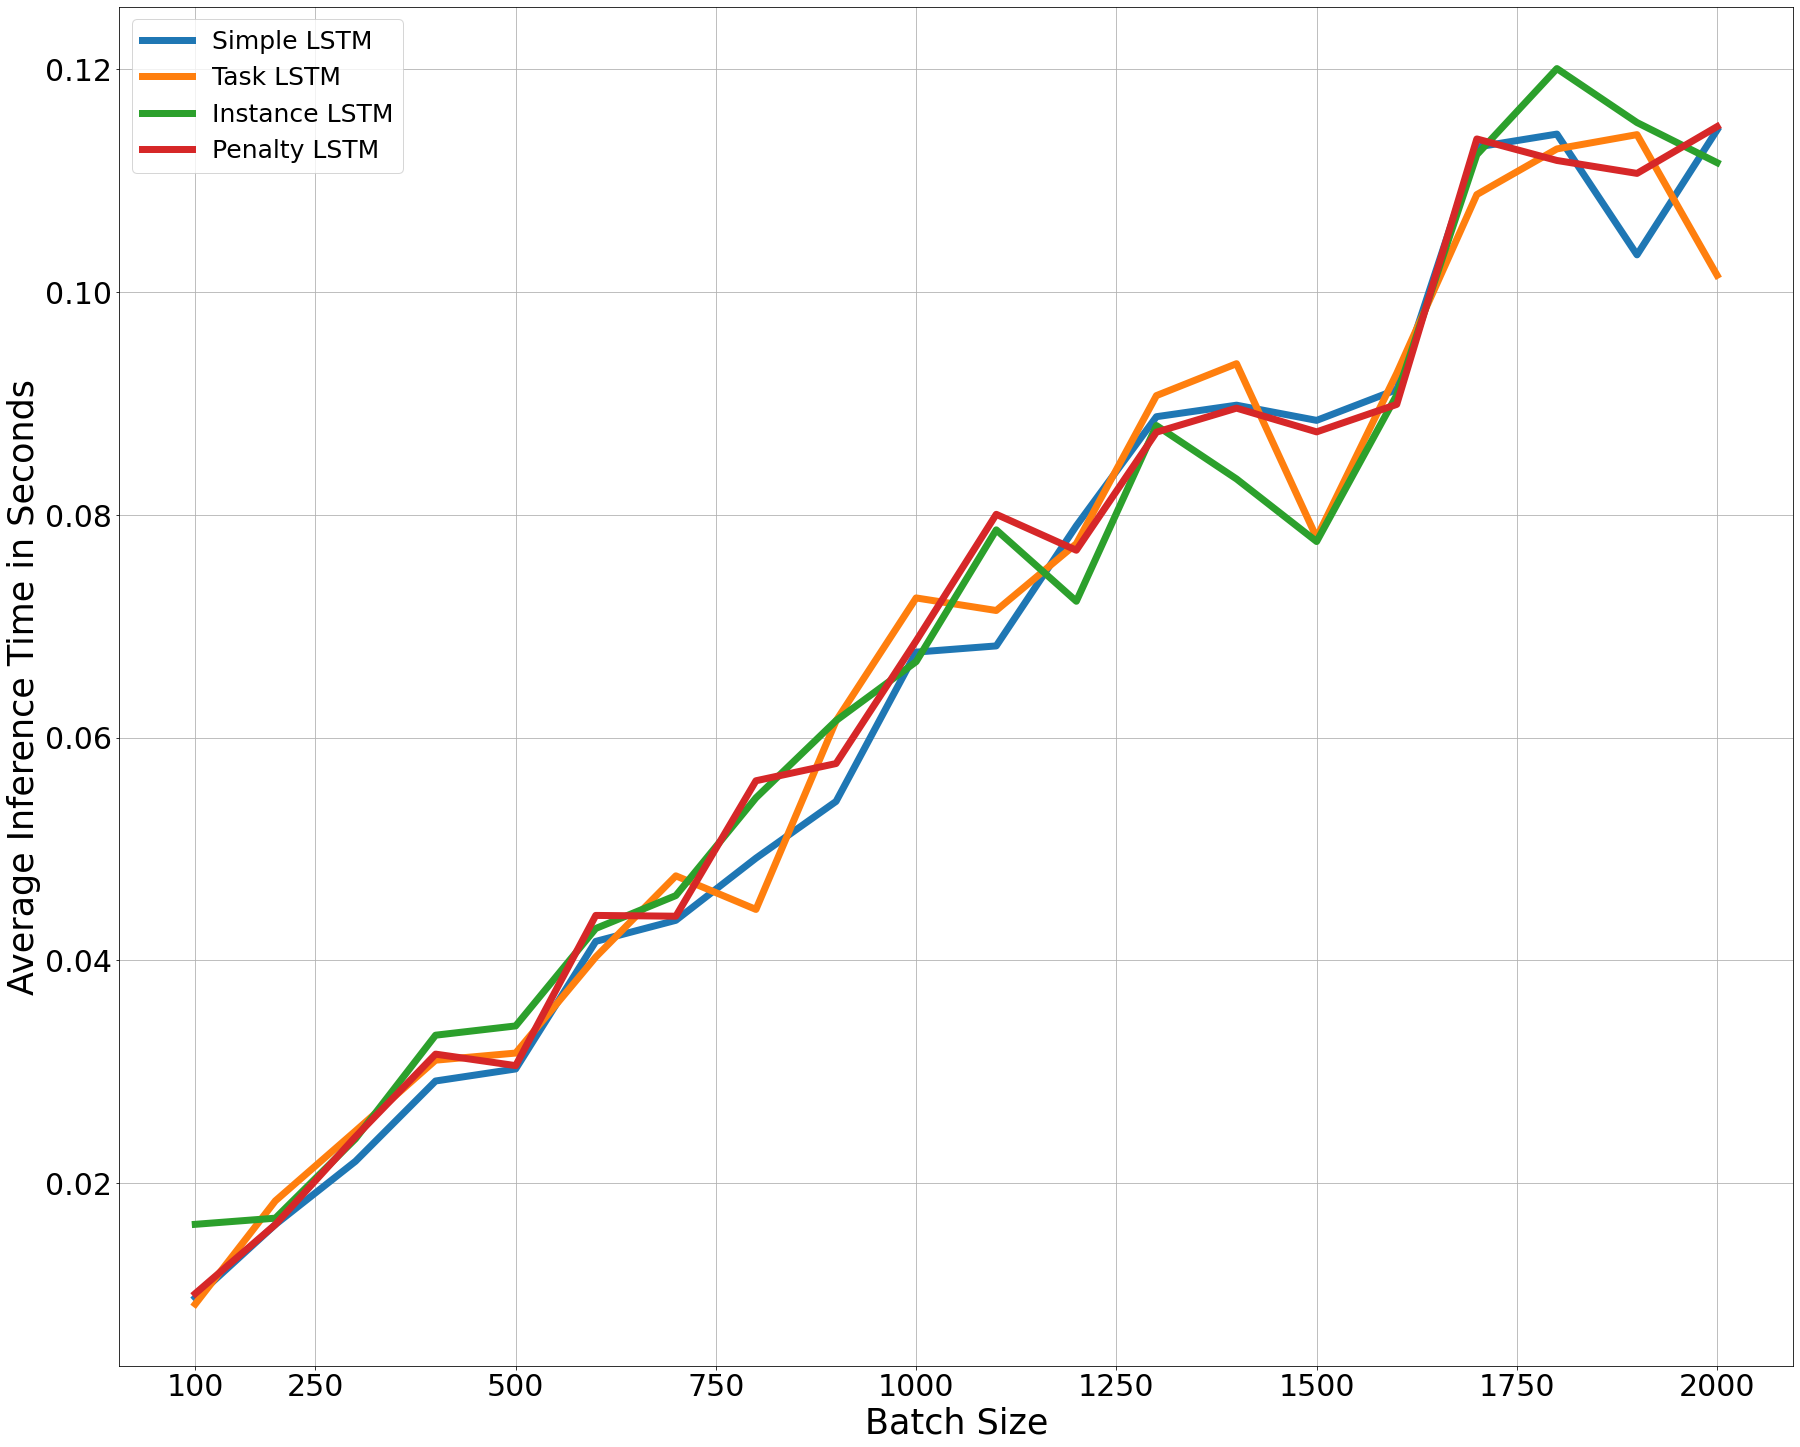
\includegraphics[width=0.99\textwidth]{figures/inference_time_batch_size.png}
    \end{figure}

    As can be seen in figure \ref{fig:average-inference-time-per-batch-size} and table \ref{tab:inference-time-of-lstm-variants} the inference times of all LSTM variants are similar regarding all batch sizes except for the Instance LSTM variant (see \ref{sec:adding-instance-knowledge-evaluation-scenarios}). 
    The Instance LSTM is the worst-performing variant in both the \emph{minimum} and \emph{maximum} values with the \emph{minimum} being $1.78$ worse than the best-performing (Task LSTM) variant. This is shown in the x-axis for the smallest batch size of $100$ in figure \ref{fig:average-inference-time-per-batch-size} by the noticeably higher line for the Instance LSTM.
    Similarly, the Instance LSTM has worse inference time performance for higher batch sizes as seen in the rightmost area of the mentioned figure by the line spike corresponding to the model.
    An explanation of why the Instance LSTM might be the worst-performing model might be the additional complexity of the feature dataset that is forwarded to the model, yet the Penalty LSTM is fed the same feature dataset and only differs in the loss function that is used to train the model.
    
    


  % \subsection{Prediction Performance Depending on Batch Size}
  % \label{sec:prediction-performance-depending-on-batch-size-evaluation-scenarios}



    % Different batch sizes
    % Different models?



  % The batch size not only influences the required training time and how much sampling data at once the model weights are updated on. The used batch size even has an impact on the prediction performance of the LSTM model.
    
  % As can be seen in the figure 
  % % \ref{fig:comparison-of-500-1000-batch-size}, 
  
  % the batch size used while training the LSTM model has a significant impact on the overall prediction performance.
  % In the figure, the training batches have the sizes 500 (orange dashed line) and 1000 (blue dashed line) elements per batch, the actual CPU utilization is shown as the black line and the CPU cores (in \%) allocated by the user are shown in the green line. While the prediction with a batch size of 500 did overestimate the CPU utilization, it has some great prediction results in the largest utilization spike, where it did come closest to the actual CPU utilization and also corrected the CPU allocation in multiple instances to either correctly use less or more CPU cores for a task.
  
  % % The training was done on a dataset size of 4000 elements total, which is only a small fraction of the actual dataset size.
  
  
  % % \begin{figure}[h!]
  % %     \centering
  % %      \includegraphics[width=\columnwidth]{figures/500_1000bs_comparison.png}
  % %     \caption{CPU Comparison of Batch Sizes 500 and 1000 - Part 1}
  % %     \label{fig:comparison-of-500-1000-batch-size}
  % % \end{figure}


  % In figure 
  % % \ref{fig:comparison-of-500-1000-batch-size-2},
  %  it is shown that the model with a batch size of 1000 is more accurately predicting lower utilization values and its overall bias in the dataset is to predict lower utilization values.
  % The model trained with batch size 500 predicts a higher CPU utilization in general but also did correctly increase/decrease the CPU utilization if the actual utilization was high/low for a longer period.

  % The opposite is observed for the model with a batch size of 1000. 
  % This model is more accurate in predicting short utilization spikes or declines compared to the model with a batch size of 500.
  
  % % \begin{figure}[h!]
  % %     \centering
  % %      \includegraphics[width=\columnwidth]{figures/500_1000bs_comparison2.png}
  % %     \caption{CPU Comparison of Batch Sizes 500 and 1000 - Part 2}
  % %     \label{fig:comparison-of-500-1000-batch-size-2}
  % % \end{figure}


  % In figure 
  % % \ref{fig:comparison-of-500-1000-batch-size-mem}, 
  % the prediction of the memory utilization is shown.
  % Opposed to the CPU utilization prediction, the model trained with the smaller batch size is biased to predict lower values in general, and the model trained with a batch size of 1000 predicted higher utilization values. Also, it was able to produce accurate predictions of the memory utilization of tasks.
  

  % TODO find out if I should keep this section
  
  % \subsection*{8. Machine-Sorted vs. Time-Stamp-Sorted Data}
  % \label{sec:machine-sorted-vs-time-stamp-sorted-data-evaluation-scenarios}

  %   All of the above evaluation scenarios were done with time-stamp sorted data. Such datasets simply refer to an ordering of the data points that were sorted by the earliest arrival time first, followed by the machine those tasks were deployed to.
  %   In the machine-sorted dataset the priority of sorting is reversed, meaning that the data points were first sorted by each machine and then all elements were sorted by the earliest arrival time for each machine. 
  %   This was done to see if there are any improvements in the prediction performance if the data set is sorted by the machine parameter first and only then sorted by the time-stamp.

    
% \section{Monitoring}



% \section{Adaptation}
